\documentclass[a4paper,11pt]{article}

% main
\usepackage[utf8]{inputenc}
\usepackage{textcomp}
\usepackage{verbatim}

\usepackage[html]{xcolor}

% tools
\usepackage{lineno}
\usepackage{hyperref}
%\usepackage{bm}
\usepackage{mathtools}
\usepackage{amssymb}
%\usepackage{algpseudocode}
\usepackage{psfrag}
\usepackage{setspace}
\usepackage{wasysym}
\usepackage[numbers]{natbib}

% style
\usepackage{graphicx}
\definecolor{darkblue}{rgb}{0,0,0.5} 
\usepackage{transparent}

% document settings
\newcommand{\loadfigure}[2][fig:nolabel]{
  \graphicspath{{#2/}}
  \def\figlabel{#1}
  \begin{figure}
  \centering

  \small

  \newcommand{\w}[1]{\textcolor{white}{#1}}
  \def\svgwidth{0.9\textwidth}

  % INKSCAPE
%% Creator: Inkscape inkscape 0.91, www.inkscape.org
%% PDF/EPS/PS + LaTeX output extension by Johan Engelen, 2010
%% Accompanies image file 'vope_pe.eps' (pdf, eps, ps)
%%
%% To include the image in your LaTeX document, write
%%   \input{<filename>.pdf_tex}
%%  instead of
%%   \includegraphics{<filename>.pdf}
%% To scale the image, write
%%   \def\svgwidth{<desired width>}
%%   \input{<filename>.pdf_tex}
%%  instead of
%%   \includegraphics[width=<desired width>]{<filename>.pdf}
%%
%% Images with a different path to the parent latex file can
%% be accessed with the `import' package (which may need to be
%% installed) using
%%   \usepackage{import}
%% in the preamble, and then including the image with
%%   \import{<path to file>}{<filename>.pdf_tex}
%% Alternatively, one can specify
%%   \graphicspath{{<path to file>/}}
%% 
%% For more information, please see info/svg-inkscape on CTAN:
%%   http://tug.ctan.org/tex-archive/info/svg-inkscape
%%
\begingroup%
  \makeatletter%
  \providecommand\color[2][]{%
    \errmessage{(Inkscape) Color is used for the text in Inkscape, but the package 'color.sty' is not loaded}%
    \renewcommand\color[2][]{}%
  }%
  \providecommand\transparent[1]{%
    \errmessage{(Inkscape) Transparency is used (non-zero) for the text in Inkscape, but the package 'transparent.sty' is not loaded}%
    \renewcommand\transparent[1]{}%
  }%
  \providecommand\rotatebox[2]{#2}%
  \ifx\svgwidth\undefined%
    \setlength{\unitlength}{842.296bp}%
    \ifx\svgscale\undefined%
      \relax%
    \else%
      \setlength{\unitlength}{\unitlength * \real{\svgscale}}%
    \fi%
  \else%
    \setlength{\unitlength}{\svgwidth}%
  \fi%
  \global\let\svgwidth\undefined%
  \global\let\svgscale\undefined%
  \makeatother%
  \begin{picture}(1,0.70675867)%
    \put(0,0){\includegraphics[width=\unitlength]{vope_pe.eps}}%
    \put(0.1193648,0.32835986){\color[rgb]{0,0,0}\makebox(0,0)[b]{\smash{$\mu_{i-1}$}}}%
    \put(0.19549212,0.32835986){\color[rgb]{1,1,1}\makebox(0,0)[b]{\smash{}}}%
    \put(0.12182045,0.56037307){\color[rgb]{0,0,0}\makebox(0,0)[b]{\smash{\w{$\pi_{i-1}$}}}}%
    \put(0.47371048,0.32835986){\color[rgb]{0,0,0}\makebox(0,0)[b]{\smash{$\mu_i$}}}%
    \put(0.82832099,0.32835986){\color[rgb]{0,0,0}\makebox(0,0)[b]{\smash{$\mu_{i+1}$}}}%
    \put(0.47703537,0.56037307){\color[rgb]{0,0,0}\makebox(0,0)[b]{\smash{\w{$\pi_i$}}}}%
    \put(0.83014525,0.56037307){\color[rgb]{0,0,0}\makebox(0,0)[b]{\smash{\w{$\pi_{i+1}$}}}}%
    \put(0.0957776,0.0813595){\color[rgb]{0,0,0}\makebox(0,0)[b]{\smash{}}}%
    \put(0.19867469,0.34932631){\color[rgb]{1,1,1}\makebox(0,0)[b]{\smash{\w{$\delta_{i-1}$}}}}%
    \put(0.55190142,0.34913153){\color[rgb]{1,1,1}\makebox(0,0)[b]{\smash{\w{$\delta_i$}}}}%
    \put(0.90678583,0.34939367){\color[rgb]{1,1,1}\makebox(0,0)[b]{\smash{\w{$\delta_{i+1}$}}}}%
    \put(0.19724716,0.03888422){\color[rgb]{0,0,0}\makebox(0,0)[b]{\smash{$\hat{\mu}_{i-1}$}}}%
    \put(0.55436625,0.03888422){\color[rgb]{0,0,0}\makebox(0,0)[b]{\smash{$\hat{\mu}_i$}}}%
    \put(0.9052044,0.03888422){\color[rgb]{0,0,0}\makebox(0,0)[b]{\smash{$\hat{\mu}_{i+1}$}}}%
    \put(0.98458269,0.49312545){\color[rgb]{0,0,0}\makebox(0,0)[rb]{\smash{\w{$\hat{\pi}_{i+1}$}}}}%
    \put(0.24528255,0.4931251){\color[rgb]{0,0,0}\makebox(0,0)[b]{\smash{\w{$\hat{\pi}_{i-1}$}}}}%
    \put(0.60324557,0.4931251){\color[rgb]{0,0,0}\makebox(0,0)[b]{\smash{\w{$\hat{\pi}_i$}}}}%
    \put(0.1206534,0.06544562){\color[rgb]{0,0,0}\makebox(0,0)[b]{\smash{$\mu_{i-1}$}}}%
    \put(0.4749991,0.06544562){\color[rgb]{0,0,0}\makebox(0,0)[b]{\smash{$\mu_i$}}}%
    \put(0.82960961,0.06544562){\color[rgb]{0,0,0}\makebox(0,0)[b]{\smash{$\mu_{i+1}$}}}%
    \put(0.61071457,0.08047097){\color[rgb]{0,0,0}\makebox(0,0)[b]{\smash{$\nu_i$}}}%
    \put(0.25549503,0.08047051){\color[rgb]{0,0,0}\makebox(0,0)[b]{\smash{$\nu_{i-1}$}}}%
    \put(0.82853716,0.45577874){\color[rgb]{1,1,1}\makebox(0,0)[b]{\smash{\w{$\Delta_{i+1}$}}}}%
    \put(0.4767936,0.45570749){\color[rgb]{1,1,1}\makebox(0,0)[b]{\smash{\w{$\Delta_i$}}}}%
    \put(0.66811134,0.46023288){\color[rgb]{0,0,0}\makebox(0,0)[b]{\smash{\w{$\gamma_i$}}}}%
    \put(0.12087086,0.45641937){\color[rgb]{1,1,1}\makebox(0,0)[b]{\smash{\w{$\Delta_{i-1}$}}}}%
    \put(0.31060081,0.45973469){\color[rgb]{0,0,0}\makebox(0,0)[b]{\smash{\w{$\gamma_{i-1}$}}}}%
    \put(0.01194257,0.65915071){\color[rgb]{0,0,0}\makebox(0,0)[lb]{\smash{1}}}%
    \put(0.01160093,0.57261339){\color[rgb]{0,0,0}\makebox(0,0)[lb]{\smash{2}}}%
    \put(0.00653804,0.49568081){\color[rgb]{0,0,0}\makebox(0,0)[lb]{\smash{3\textsf{A}}}}%
    \put(0.00653845,0.34751437){\color[rgb]{0,0,0}\makebox(0,0)[lb]{\smash{3\textsf{B}}}}%
    \put(0.0113686,0.21454449){\color[rgb]{0,0,0}\makebox(0,0)[lb]{\smash{4}}}%
    \put(0.00651485,0.1385617){\color[rgb]{0,0,0}\makebox(0,0)[lb]{\smash{5\textsf{A}}}}%
    \put(0.00651485,0.07872525){\color[rgb]{0,0,0}\makebox(0,0)[lb]{\smash{5\textsf{B}}}}%
    \put(0.01169903,0.02743687){\color[rgb]{0,0,0}\makebox(0,0)[lb]{\smash{6}}}%
    \put(0.22864656,0.60855135){\color[rgb]{0.62352941,0,0.52941176}\makebox(0,0)[b]{\smash{$\alpha_{i-1,i}^2$}}}%
    \put(0.56974768,0.60855091){\color[rgb]{0.62352941,0,0.52941176}\makebox(0,0)[lb]{\smash{$\alpha_{i,i+1}^2$}}}%
  \end{picture}%
\endgroup%

  \caption{Overview of prediction error computation in \textsf{VOPE} coupling.}
  \label{\figlabel}
\end{figure}
}
\title{Message Passing in the Hierarchical Gaussian Filter}

\begin{document}

\maketitle

\section{The generative model of the HGF: Volatility vs. value coupling}

In the generative model of the HGF, (hidden) states of the world perform Gaussian random walks in time and can produce outcomes which are perceived by an observer as inputs. States can influence each other via volatility coupling or via value coupling.\\

In the classical 3-level binary HGF as presented in \cite{Mathys2011}, the two states of interest, $x_2$ and $x_3$ are coupled to each other via volatility coupling, which means that for state $x_2$, the mean of the Gaussian random walk on trial $k$ is given by its previous value $x_2^{(k-1)}$, while the step size (or variance) depends on the previous value of the higher level state, $x_3^{(k-1)}$:

\begin{equation}
    x_2^{(k)} \sim \mathcal{N}(x_2^{(k)} | x_2^{(k-1)}, \, f(x_3^{(k-1)})), 
\end{equation} 

where the exact dependency is of the form

\begin{equation}
    f(x_3^{(k-1)}) = \exp(\kappa_2 x_3^{(k-1)} + \omega_2).
\end{equation}

However, a higher-level state can also have influence on a lower-level state by influencing its mean. In that case, the mean of the Gaussian random walk at one level is a function not only of its own previous value, but also the previous value of the higher-level state (with step size either constant or a function of another state):

\begin{equation}
    x_2^{(k)} \sim \mathcal{N}(x_2^{(k)} | x_2^{(k-1)} + \alpha_{4,2} x_4^{(k-1)}, \, exp(\omega_2)),
\end{equation}

which means constant step size, or

\begin{equation}
    x_2^{(k)} \sim \mathcal{N}(x_2^{(k)} | x_2^{(k-1)} + \alpha_{4,2} x_4^{(k-1)}, \, \exp(\kappa_2 x_3^{(k-1)} + \omega_2)).
\end{equation}

In other words, any given state in the world can be modelled as having a volatility parent state, a value parent state, or both, or none (in which case it evolves as a Gaussian random walk around its previous value with fixed step size). Consequently, when inferring on the evolution of these states, the exact update equations (which include the computation of new predictions, posterior values, and prediction errors, and represent an approximate inversion of this generative model, see \cite{Mathys2011}) depend on the nature of the coupling of a given state with its parent and children states.\\

In figure \ref{fig:genmod} we have drawn an example setup with six different environmental states and one outcome. Here, we have denoted states that function as value parents for other states as $x_i$, and states that function as volatility parents as $\check{x}_i$. Volatility coupling is depicted by curvy arrows, value coupling by straight arrows, and observable outcomes are linked to their hidden states via double arrows. \\

For the example illustrated in figure \ref{fig:genmod}, the following equations describe the generative model:

\begin{align}
    u^{(k)}             &\sim \mathcal{N}(u^{(k)} | x_1^{(k)}, \, &\sigma_u)\\
    x_1^{(k)}           &\sim \mathcal{N}(x_1^{(k)} | x_1^{(k-1)} + \alpha_{2,1} x_2^{(k-1)}, \, &\exp(\kappa_1 \check{x}_1^{(k-1)} + \omega_1))\\
    \check{x}_1^{(k)}   &\sim \mathcal{N}(\check{x}_1^{(k)} | \check{x}_1^{(k-1)} + \alpha_{3,\check{1}} x_3^{(k-1)}, \, &\exp(\omega_{\check{1}}))\\
    x_2^{(k)}           &\sim \mathcal{N}(x_2^{(k)} | x_2^{(k-1)}, \, &\exp(\kappa_2 \check{x}_2^{(k-1)} + \omega_2))\\
    \check{x}_2^{(k)}   &\sim \mathcal{N}(\check{x}_2^{(k)} | \check{x}_2^{(k-1)}, \, &\exp(\omega_{\check{2}}))\\
    x_3^{(k)}           &\sim \mathcal{N}(x_3^{(k)} | x_3^{(k-1)}, \, &\exp(\kappa_3 \check{x}_3^{(k-1)} + \omega_3))\\
    \check{x}_3^{(k)}   &\sim \mathcal{N}(\check{x}_3^{(k)} | \check{x}_3^{(k-1)}, \, &\exp(\omega_{\check{3}})).
\end{align}

Note that in this example, all states that are value parents of other states (or outcomes) have their own volatility parent, while states that are volatility parents to other nodes either have a value parent (as state $\check{x}_1$), or no parents (as states $\check{x}_2$ and $\check{x}_3$). This is deliberately so, and we will see these two motifs - every state of a hierarchy has its own volatility estimation, and volatility states only have value parents - reappear in the following chapters.
\section{Computations of Nodes in the HGF}
In the HGF, each node has to perform several computations within an experimental trial, which can be ordered in time as shown in the box:
\vspace{1cm}

\noindent
\fbox{
  \begin{minipage}{0.7\textwidth}
  	\linespread{2}
  	\textsc{Node} \textit{i} \textsc{at trial} \textit{k}\\
  	\vspace{0.2cm}\\
    $\leftarrow$ \texttt{receive} $\mathrm{PE}^{(k)}_{i-1}$
                from $\mathrm{node}_{i-1}$\\
    %\vspace{2pt}\\
    
    \textsf{UPDATE step}\\
    \hspace*{0.2cm} \texttt{compute} $\mathrm{posterior}^{(k)}_i$ \\
    \hspace*{0.2cm} \textit{given:} $\mathrm{PE}^{(k)}_{i-1}$ and 
    								$\mathrm{prediction}^{(k)}_i$
	\vspace{4pt}\\
    $\rightarrow$ \texttt{send} $\mathrm{posterior}^{(k)}_i$
    						 to $\mathrm{node}_{i-1}$
    \vspace{0.2cm}\\
    
    \textsf{PE step} \\
    \hspace*{0.2cm} \texttt{compute} $\mathrm{PE}^{(k)}_i$ \\
    \hspace*{0.2cm} \textit{given:} $\mathrm{prediction}^{(k)}_i$ and 
    								$\mathrm{posterior}^{(k)}_i$
	\vspace{4pt}\\
    $\rightarrow$ \texttt{send} $\mathrm{PE}^{(k)}_i$
    						 to $\mathrm{node}_{i+1}$\\
    $\leftarrow$ \texttt{receive} $\mathrm{posterior}^{(k)}_{i+1}$
    			from $\mathrm{node}_{i+1}$
    \vspace{0.2cm}\\

    \textsf{PREDICTION step} \\
    \hspace*{0.2cm} \texttt{compute} $\mathrm{prediction}^{(k+1)}_i$ \\
    \hspace*{0.2cm} \textit{given:} $\mathrm{posterior}^{(k)}_i$ and 
    								$\mathrm{posterior}^{(k)}_{i+1}$
	\vspace{4pt}\\
  \end{minipage}
}

\vspace{1cm}
\noindent
The exact computations in each step depend on the nature of the coupling (\textsf{VAPE} vs. \textsf{VOPE}) with the parent and children nodes. Critically, it is not only the PEs that are sent upwards, but depending on the coupling also other quantities need to signalled.

%\newpage
\section{Computations for VAPE coupling}
The exact computations of the \textsf{UPDATE step} depend on the nature of the coupling with the child node(s), while both the \textsf{PE step} and the \textsf{PREDICTION step} depend on the coupling with the parent node(s).

\subsection{Update Step}
If Node~$i$ is the value parent of Node $i-1$, then the following update equations apply to Node~$i$:
\vspace{0.5cm}

\noindent
\fbox{
\begin{minipage}{\textwidth}

\begin{align}
\pi_i^{(k)} &= \hat{\pi}_i^{(k)} 
			+ \alpha_{i-1,i}^2 \hat{\pi}_{i-1}^{(k)}\\
\mu_i^{(k)} &= \hat{\mu}_i^{(k)} 
			+ \frac{\alpha_{i-1,i}^2 \hat{\pi}_{i-1}^{(k)}} {\alpha_{i-1,i}^2 \hat{\pi}_{i-1}^{(k)} + \hat{\pi}_{i}^{(k)}} \delta_{i-1}^{(k)}
\end{align}			
\vspace{1pt}

\end{minipage}
}%end:fbox
\vspace{0.5cm}

\noindent
We note here that we can let the update of the precision happen first, and therefore use it for the update of the mean:
\vspace{0.5cm}

\noindent
\fbox{
\begin{minipage}{\textwidth}

\begin{align}
\pi_i^{(k)} &= \hat{\pi}_i^{(k)} 
			+ \alpha_{i-1,i}^2 \hat{\pi}_{i-1}^{(k)}\\
\mu_i^{(k)} &= \hat{\mu}_i^{(k)} 
			+ \frac{\alpha_{i-1,i}^2 \hat{\pi}_{i-1}^{(k)}} {\pi_i^{(k)}} \delta_{i-1}^{(k)}
\end{align}			
\vspace{1pt}

\end{minipage}
}%end:fbox
\vspace{0.5cm}

\noindent
In sum, at the time of the update, Node~$i$ needs to have access to the following quantities:

\begin{description}
\item[Its own predictions:]  	$\hat{\mu}_i^{(k)}$, $\hat{\pi}_i^{(k)}$
\item[Coupling strength:] 		$\alpha_{i-1,i}$
\item[From level below:]		$\delta_{i-1}^{(k)}$, $\hat{\pi}_{i-1}^{(k)}$
\end{description}

All of these are available at the time of the update. Node~$i$ therefore only needs to receive the PE and the predicted precision from the level below to perform its update.

\subsection{Prediction Error Step}
We will assume in the following, that Node~$i$ is the value child of Node $i+1$. Then the following quantities have to be sent up to Node $i+1$ (cf. necessary information from level below in a value parent):

\begin{description}
\item[Predicted precision:] 	$\hat{\pi}_{i}^{(k)}$
\item[Prediction error:]		$\delta_{i}^{(k)}$
\end{description}

Node~$i$ has already performed the \textsf{PREDICTION step} on the previous trial, so it has already computed the predicted precision of the current trial,~$\hat{\pi}_{i}^{(k)}$. Hence, in the \textsf{PE step}, it needs to perform only the following calculation:
\vspace{0.5cm}

\noindent
\fbox{
\begin{minipage}{\textwidth}

\begin{equation}
\delta_i^{(k)} 	= \mu_i^{(k)} - \hat{\mu}_i^{(k)}
\end{equation}			
\vspace{1pt}

\end{minipage}
}%end:fbox
\vspace{0.5cm}

\noindent


\subsection{Prediction Step}
Still assuming that Node~$i$ is the value child of Node $i+1$, the \textsf{PREDICTION step} consists of the following computations:
\vspace{0.5cm}

\noindent
\fbox{
\begin{minipage}{\textwidth}

\begin{align}
\hat{\mu}_i^{(k+1)} 	&= \mu_i^{(k)} + \alpha_{i,i+1} \mu_{i+1}^{(k)}\\
\hat{\pi}_i^{(k+1)} 	&= \frac{1}{\frac{1}{\pi_i^{(k)}} + \nu_i^{(k+1)} }
\end{align}			
\vspace{1pt}

\end{minipage}
}%end:fbox
\vspace{0.5cm}

\noindent
with
\begin{equation*}
\nu_i^{(k+1)} = \exp(\omega_i).
\end{equation*}

Note that if Node~$i$ additionally has a \textsf{VOPE} parent node, the estimated volatility $\nu_i^{(k+1)}$ that enters the precision update would also depend on the posterior mean of that volatility parent (cf. \textsf{PREDICTION step} for \textsf{VOPE} coupling).\\

In general, the prediction of the mean will depend only on whether Node~$i$ has a value parent or not, whereas the prediction of the precision only depends on whether Node~$i$ has a volatility parent or not. \\

However, without a volatility parent node, the estimated volatility only depends on the node's own learning rate $\omega_i$, i.e., it is a constant. We can therefore simply write:
\vspace{0.5cm}

\noindent
\fbox{
\begin{minipage}{\textwidth}

\begin{align}
\hat{\mu}_i^{(k+1)} 	&= \mu_i^{(k)} + \alpha_{i,i+1} \mu_{i+1}^{(k)}\\
\hat{\pi}_i^{(k+1)} 	&= \frac{1}{\frac{1}{\pi_i^{(k)}} + \exp(\omega_i) }
\end{align}			
\vspace{1pt}

\end{minipage}
}%end:fbox
\vspace{0.5cm}

\noindent

Thus, the \textsf{PREDICTION step} only depends on knowing the node's own posteriors and receiving the value parent's posterior in time before the new input arrives.
%\newpage
\section{Computations for VOPE coupling}
As in the case of \textsf{VAPE} coupling, the exact computations of the \textsf{UPDATE step} depend on the nature of the coupling with the child node(s), while both the \textsf{PE step} and the \textsf{PREDICTION step} depend on the coupling with the parent node(s).\\

To describe the computations entailed by \textsf{VOPE} coupling, we will introduce two changes to the notation. First of all, we will express the volatility PE, or \textsf{VOPE}, as a function of the previously defined value PE, or \textsf{VAPE}. That means from now on, we will use the character $\delta_i$ only for \textsf{VAPE}s:

\begin{equation}
	\delta_i^{(k)} \equiv \delta_i^{(k, VAPE)} = \mu_i^{(k)} - \hat{\mu}_i^{(k)},
\end{equation}

and introduce a new character $\Delta_i$ for \textsf{VOPE}s, which we define as 

\begin{equation}
  \begin{split}
    \Delta_i^{(k)} \equiv \delta_i^{(k, VOPE)} &= \frac{ \frac{1}{\pi_{i}^{(k)}} + (\mu_i^{(k)} - \hat{\mu}_i^{(k)})^2 }{ \frac{1}{\pi_{i}^{(k-1)}} + \nu_{i}^{(k)} } - 1 \\
    &= \hat{\pi}_i^{(k)} \left( \frac{1}{\pi_{i}^{(k)}} + (\mu_i^{(k)} - \hat{\mu}_i^{(k)})^2 \right) - 1 \\
    &= \hat{\pi}_i^{(k)} \left( \frac{1}{\pi_{i}^{(k)}} + (\delta_i^{(k)})^2 \right) - 1 \\
    &=  \frac{\hat{\pi}_i^{(k)}}{\pi_{i}^{(k)}} + \hat{\pi}_i^{(k)} (\delta_i^{(k)})^2 - 1. \\
  \end{split} 
\end{equation}

Note that from the first to the second line, we have used the following definition:

\begin{equation*}
\hat{\pi}_{i-1}^{(k)} = \frac{1}{ \frac{1}{\pi_{i-1}^{(k-1)}} + \nu_{i-1}^{(k)} }.
\end{equation*}

This ensures that a given node does not need to have access to the posterior precision from the level below: $\pi_{i-1}^{(k-1)}$, which facilitates implementation.\\

In sum, we are introducing a second prediction error unit $\Delta_i$ which is concerned with deviations from predicted uncertainty and is informed by value prediction errors and other estimates of uncertainty. It is this prediction error - a function of the unweighted (squared) value prediction error with a new precision weight - which communicates between a level's nodes and a level's volatility parent's nodes.\\

Second, we will introduce another quantity, which we term the (auxiliary) expected precision

\begin{equation}
  \gamma_i^{(k)} = \nu_i^{(k)} \hat{\pi}_i^{(k)},
\end{equation}

which will be computed as part of the \textsf{PREDICTION step} and only serves to simplify the equations and the corresponding message passing.

\subsection{Update Step}
If Node $i$ is the volatility parent of Node $i-1$, then the following update equations apply to Node $i$:

\begin{align*}
\pi_i^{(k)} &= \hat{\pi}_i^{(k)} 
			+ \frac{1}{2}(\kappa_{i-1} \nu_{i-1}^{(k)} \hat{\pi}_{i-1}^{(k)})^2
			* (1 + (1 - \frac{1}{\pi_{i-1}^{(k-1)} \nu_{i-1}^{(k)}}) 
			\delta_{i-1}^{(k)})\\
			&= \hat{\pi}_i^{(k)} 
			+ \frac{1}{2}(\kappa_{i-1} \nu_{i-1}^{(k)} \hat{\pi}_{i-1}^{(k)})^2
			* (1 + (2 - \frac{1}{\hat{\pi}_{i-1}^{(k)} \nu_{i-1}^{(k)}}) 
			\delta_{i-1}^{(k)})\\
\mu_i^{(k)} &= \hat{\mu}_i^{(k)} 
			+ \frac{1}{2}\kappa_{i-1} \nu_{i-1}^{(k)} 
			\frac{\hat{\pi}_{i-1}^{(k)}}{\pi_{i}^{(k)}} \delta_{i-1}^{(k)},
\end{align*}			

where we have again used the definition of the predicted precision $\hat{\pi}_{i-1}^{(k)}$ to derive an expression for the posterior precision from the previous trial $\pi_{i-1}^{(k-1)}$:

\begin{align*}
\hat{\pi}_{i-1}^{(k)} 			  &= \frac{1}{ \frac{1}{\pi_{i-1}^{(k-1)}}
								  + \nu_{i-1}^{(k)} }\\
\Leftrightarrow \pi_{i-1}^{(k-1)} &= \frac{1}{ \frac{1}{\hat{\pi}_{i-1}^{(k)}}
					  			  - \nu_{i-1}^{(k)} }.
\end{align*}

With the changes from above, namely the definitions of the \textsf{VOPE} $\Delta_i$ and the expected precision $\gamma_i^{(k)}$, the update equations for the precision and the mean in volatility coupling simplify to:
\vspace{0.5cm}

\noindent
\fbox{
\begin{minipage}{\textwidth}

\begin{align}
\pi_i^{(k)} &= \hat{\pi}_i^{(k)} 
			+ \frac{1}{2} (\kappa_{i,i-1} \gamma_{i-1}^{(k)})^2 
			+ (\kappa_{i,i-1} \gamma_{i-1}^{(k)})^2 \Delta_{i-1}^{(k)} 
			- \frac{1}{2} \kappa_{i,i-1} \gamma_{i-1}^{(k)} \Delta_{i-1}^{(k)}\\
\mu_i^{(k)} &= \hat{\mu}_i^{(k)} 
			+ \frac{1}{2} \frac{\kappa_{i,i-1} \gamma_{i-1}^{(k)}}{\pi_i^{(k)}} \Delta_{i-1}^{(k)}
\end{align}			
\vspace{1pt}

\end{minipage}
}%end:fbox
\vspace{0.5cm}

\noindent
Therefore, at the time of the update, Node $i$ needs to have access to the following quantities:

\begin{description}
\item[Its own predictions:]  	$\hat{\mu}_i^{(k)}$, $\hat{\pi}_i^{(k)}$
\item[Coupling strength:] 		$\kappa_{i,i-1}$
\item[From level below:]		$\Delta_{i-1}^{(k)}$, $\gamma_{i-1}^{(k)}$
\end{description}


\subsection{Prediction Error Step}
The exact computation of the prediction error depends, like the computation of the new prediction, on the nature of the coupling with the parent nodes. We will therefore assume in the following, that Node $i$ is the volatility child of Node $i+1$. Then the following quantities have to be sent up to Node $i+1$ (see also necessary information from level below in a volatility parent):

\begin{description}
\item[Expected precision:] 		$\gamma_{i}^{(k)}$
\item[Prediction error:]		$\Delta_{i}^{(k)}$
\end{description}

Node $i$ has already performed the \textsf{PREDICTION step} on the previous trial, so it has already computed the predicted precision, $\hat{\pi}_{i}^{(k)}$, and the volatiliy estimate, $\nu_i^{(k)}$, and out of these the expected precision, $\gamma_{i}^{(k)}$, for the current trial. Hence, in the \textsf{PE step}, it needs to perform only the following calculations:
\vspace{0.5cm}

\noindent
\fbox{
\begin{minipage}{\textwidth}

\begin{align}
\delta_i^{(k)} &= \mu_i^{(k)} - \hat{\mu}_i^{(k)}\\
\Delta_i^{(k)} &= \frac{\hat{\pi}_i^{(k)}}{\pi_{i}^{(k)}} + \hat{\pi}_i^{(k)} (\delta_i^{(k)})^2 - 1.
\end{align}			
\vspace{1pt}

\end{minipage}
}%end:fbox
\vspace{0.5cm}

\noindent

\subsection{Prediction Step}
Still assuming that Node $i$ is the volatility child of Node $i+1$, the \textsf{PREDICTION step} consists of the following simple computations:
\vspace{0.5cm}

\noindent
\fbox{
\begin{minipage}{\textwidth}

\begin{align}
\hat{\mu}_i^{(k+1)} 	&= \mu_i^{(k)}\\
\nu_i^{(k+1)} 			&= \exp(\kappa_i \mu_{i+1}^{(k)} + \omega_i)\\
\hat{\pi}_i^{(k+1)} 	&= \frac{1}{\frac{1}{\pi_i^{(k)}} + \nu_i^{(k+1)} }\\
\gamma_i^{(k+1)} 			&= \nu_i^{(k+1)} \hat{\pi}_i^{(k+1)}
\end{align}			
\vspace{1pt}

\end{minipage}
}%end:fbox
\vspace{0.5cm}

\noindent
Thus, the prediction for trial $k+1$ depends again only on receiving the posterior mean of Node $i+1$ on trial $k$, and knowing the Node's own posteriors.\\

Note that if Node~$i$ additionally has a \textsf{VAPE} parent node, the prediction of the new mean, $\hat{\mu}_i^{k+1}$ would also depend on the posterior mean of that value parent (cf. \textsf{PREDICTION step} for \textsf{VAPE} coupling).
%\newpage
\section{Implementation HGF coupling}

If we assume that a cortical column consists of units (i.e., sub-populations of neurons), one for each computational step, then the computations for \textsf{VAPE coupling} as well as for \textsf{VOPE coupling} could be implemented as sketched in Figure 1.

\begin{figure}[h]
	\includegraphics[width = \textwidth]{figures/impl/fig2}
	\caption{Example implementation of the coupling between cortical columns in the HGF. Figure shows two cortical columns that could be coupled to each other via VAPE or VOPE coupling. In each case, the messages passed along the connections and the computations within the nodes would differ according to the equations presented in the previous chapters.}
\end{figure}

A few points to note here:
\begin{itemize}
\item In this implementation, we assume that the estimated volatility, $\nu_i^{k}$, is computed within the \textsf{Prediction} unit. This is motivated by the equations presented above and the fact that this unit receives information about the updated quantities (posterior means and precisions) from the level above.
\item Similarly, the only unit that needs to know the value of a node's tonic learning rate, $\omega_i$, is the \textsf{Prediction} unit. Therefore, this parameter could be implemented in terms of self-connections or interneurons within that neuronal population.
\item A noteworthy arrow in this picture is the one from the \textsf{Prediction} unit of one node to the \textsf{Update} unit of its parent node. This seems to violate the classical assumptions that while top-down connections signal predictions, bottom-up connections would only signal prediction errors. Due to the update equations in the HGF, however, any given parent node needs access to the predicted precision from its child node to perform an update. To avoid this arrow, we could also assume that the \textsf{Prediction} unit sends the predicted precision to the \textsf{PE} unit of the same node, which then sends this quantity up to the \textsf{Update} unit of the parent node. However, this seems more complicated for two reasons: First, the \textsf{PE} unit doesn't actually need this quantity to perform its computation. Secondly, the PE is computed only somewhat after the prediction of the current trial (which is already computed after the previous trial). Thus, the two signals would be sent up at different times.
\item Note that we did not distinguish between the computational steps \textsf{Prediction} and \textsf{Update} for the mean versus for the precision here. It is likely however, that these would be encoded in separate neuronal populations. Also, the implementation of VAPE and VOPE parents might differ. We will address these specifications below in comparison to classical predictive coding schemes.
\end{itemize}
%\newpage

\section{Relation to Predictive Coding}

In this section, we consider an implementation of the message passing implicated by the HGF which is as close as possible to current proposals of neural architectures for predictive coding \cite{Shipp2016}.\\

We will separately consider \textsf{VAPE} and \textsf{VOPE} coupling and realize that the message passing for \textsf{VAPE} coupling is almost equivalent to the proposed PC architecture, while the \textsf{VOPE} coupling comes with more challenges, simply because it hasn't been addressed in detail in existing PC proposals on neural architecture.

\loadfigure[fig:vaall]{figures/vape_all}

\subsection{VAPE coupling}

Figure \ref{fig:vaall} sketches a possible architecture implementing all computations involved in \textsf{VAPE} coupling for three example cortical regions (levels). The assignment of neural elements to cortical layers follows the proposal in in figure 3 of \cite{Shipp2016}. For example, we've placed all precision-related nodes into the upper layers, while expectations and predictions of the mean live in intermediate and deep layers, respectively. In the following, we go through the different computational steps and note differences to the proposal for predictive coding.

For the \textsf{PE} step, we have the following computation:

\begin{equation}
	\delta_i^{(k)} = \mu_i^{(k)} - \hat{\mu}_i^{(k)}.
\end{equation}

\loadfigure[fig:vape]{figures/vape_pe}

The message passing implicated is depicted in figure \ref{fig:vape} and is in line with PE computations as suggested by \cite{Shipp2016}.

In the \textsf{Update} step, the posterior estimates of mean an variance are given by:

\begin{equation}
	\mu_i^{(k)} = \hat{\mu}_i^{(k)} + \frac{\alpha_{i-1,i}^2 \hat{\pi}_{i-1}^{(k)}}{\pi_i^{(k)}} \delta_{i-1}^{(k)}
\end{equation}

and

\begin{equation}
	\pi_i^{(k)} = \hat{\pi}_i^{(k)} + \alpha_{i-1,i}^2 \hat{\pi}_{i-1}^{(k)}.
\end{equation}

A possible message passing implementation for these updates is shown in figure \ref{fig:vaupdate}. There are two important differences to \cite{Shipp2016} to note here.\\

\loadfigure[fig:vaupdate]{figures/vape_update}

First, in \textsf{PC} proposal, the update of the mean $\mu_i$ is driven both by the lower-level PE $\delta_{i-1}$ and the PE on the level itself, $\delta_i$, which mediates the influence of the empirical prior, or the prediction, on the mean. 

In the HGF equations, we do not have this negative feedback loop from $\delta_i$ to $\mu_i$. Instead, the prediction $\hat{\mu}_i$ has a direct influence on $\mu_i$ (see equations above), hence the arrow from the $\hat{\mu}_i$ node to the $\mu_i$ node in figure \ref{fig:vaupdate}. 

However, by considering the within-trial temporal evolution of the $\mu_i$ node, we can get the same feedback loop. Noting that $\mu_i$ as computed in the above equation will be the endpoint of the update, i.e., the equilibrium value to which the node should stabilize at the end of trial $k$, we can, in the style of \cite{Bogacz2017}, propose the following temporal evolution:

\begin{equation}
	\dot{\mu}_i^{(k)} = \hat{\mu}_i^{(k)} + \frac{\alpha_{i-1,i}^2 \hat{\pi}_{i-1}^{(k)}}{\pi_i^{(k)}} \delta_{i-1}^{(k)} - \mu_i^{(k)}
\end{equation}

Clearly, a node with this dynamic converges to the required posterior value, which can be seen by setting $\dot{\mu}_i$ to zero. Now we note that

\begin{equation}
	\dot{\mu}_i^{(k)} = \frac{\alpha_{i-1,i}^2 \hat{\pi}_{i-1}^{(k)}}{\pi_i^{(k)}} \delta_{i-1}^{(k)} - \mu_i^{(k)} + \hat{\mu}_i^{(k)}
\end{equation}

can be summarized as 

\begin{equation}
	\dot{\mu}_i^{(k)} = \frac{\alpha_{i-1,i}^2 \hat{\pi}_{i-1}^{(k)}}{\pi_i^{(k)}} \delta_{i-1}^{(k)} - \delta_i^{(k)}.
\end{equation}

Following this logic, we could also place the arrow between $\delta_i$ and $\mu_i$. The exercise of writing down the within-trial temporal dynamics of the nodes will be repeated below for all nodes, which results in equations for within-trial network dynamics. These can be used to simulate within-trial responses of all nodes, examining network stability, and predicting neural dynamics which could for example be compared with electrophysiological data. 

The second difference to the \textsf{PC} proposal is rather irreducible. As already mentioned in the previous section, the messages sent up to parent nodes do not only consist of prediction errors or their precision weights. Instead, to update the precision node $\pi_i$, node $i$ also needs access to the prediction precision $\hat{\pi}_{i-1}$ from the level below. This is reflected in the violet arrow travelling from superficial layers of level $i$ to level $i+1$. 

Finally, in the \textsf{Prediction} step, we have:

\begin{equation}
	\hat{\mu}_i^{(k+1)} = \mu_i^{(k)} + \alpha_{i,i+1} \mu_{i+1}^{(k)}
\end{equation}

and

\begin{equation}
	\hat{\pi}_i^{(k+1)} = \frac{1}{\frac{1}{\pi_i^{(k)}} + \exp(\omega_i)}.
\end{equation}

\loadfigure[fig:vaprediction]{figures/vape_prediction}

This again seems unproblematic, although the arrow from $\mu_i$ to $\hat{\mu}_i$ would not appear in the classical \textsf{PC} architecture. Also, we've placed the predicted precision $\hat{\pi}$ in the superficial layers here, for convenience, as it interacts only with the posterior precision $\pi$ and acts as a weight on the prediction error, and also inaccordance with \cite{Shipp2016}, where precision signals arise from layers 2 and 3A. 

\subsection{VOPE coupling}
For volatility parents, we propose the following: Each level of a cortical hierarchy implements its own volatility parent in superficial layers. Coupling across layers is exclusively value-related. This means that having a volatility parent is nothing more but a more sophisticated way of predicting and updating a level's precision estimates. \\

This setup excludes volatility parents of volatility parents. However, it allows a cortical hierarchy where higher levels predict either the mean, or the volatility, of lower levels, both via value coupling. In other words, any given level receives top-down predictions not only about its mean, but also about its volatility, which is implemented as the mean of its volatility parent.\\

Due to this proposal, we slightly change the notation from here on. Level $i$ from now on refers to hierarchical level within a cortical hierarchy. Nodes on this level comprise the 'original' nodes $\mu_i$, $\pi_i$, $\hat{\mu}_i$, $\hat{\pi}_i$, and $\delta_i$, but also all the nodes belonging to a volatility parent of these nodes, which we now denote as $\check{\mu}_i$, $\check{\pi}_i$, $\hat{\check{\mu}}_i$, $\hat{\check{\pi}}_i$, and $\check{\delta}_i$. Here, $\check{\delta}_i$ refers to the value prediction error about the mean of the volatility, $\check{\mu}_i$. \\

We also introduce a new character for the \textsf{VOPE}, $\Delta_i$, which we write as a function of the \textsf{VAPE}, $\delta_i$, of level $i$. This PE is what communicates between a level's nodes and a level's volatility parent's nodes (see below for equations and visualizations). 

\loadfigure[fig:voall]{figures/vope_all}
\loadfigure[fig:withvol]{figures/zoom_vape_with_vope}

Figure \ref{fig:voall} displays one proposal for this setup, where we've zoomed in to a level $i$ of the cortical hierarchy (and a value parent $i+1$) and added its volatility parent to the superficial layers. An alternative implementation of this idea is displayed in figure \ref{fig:withvol}. Here, only the precision-related computations of the volatility parent are placed in the superficial layers, while the corresponding prediction errors, $\Delta_i$ and $\check{\delta}_i$ as well as the actual volatility estimate $\check{\mu}_i$ live in middle layers, and the prediction of the volatility estimate, $\hat{\check{\mu}}_i$, lives in layer 6. This setup stresses the structural similarities to the message passing entailed by mean coupling. Moreover, using this setup, we can now depict how a higher cortical level $i+1$ would serve as a value parent to the volatility estimate in level $i$ - instead of predicting the mean - by simply exchanging the arrows between the levels as shown in figure \ref{fig:volparent}. 

\loadfigure[fig:volparent]{figures/zoom_vope}

Note that in principle, both the mean $\mu_i$ as well as the volatility estimate $\check{\mu}_i$ of a given level could have (one or more) value parents in higher cortical areas. This allows for both separate and combined higher-level prediction of both the precision and the mean of level $i$.

We now turn to the equations for the within-level volatility node. The volatility prediction error (\textsf{VOPE}) can be written as a function of the value prediction error (\textsf{VAPE}), where we now use $\delta_i$ only for \textsf{VAPE}s:

\begin{equation}
	\delta_i^{(k)} \equiv \delta_i^{(k, VAPE)} = \mu_i^{(k)} - \hat{\mu}_i^{(k)},
\end{equation}

We define the \textsf{VOPE} as 

\begin{equation}
  \begin{split}
    \Delta_i^{(k)} \equiv \delta_i^{(k, VOPE)} &= \frac{ \frac{1}{\pi_{i}^{(k)}} + (\mu_i^{(k)} - \hat{\mu}_i^{(k)})^2 }{ \frac{1}{\pi_{i}^{(k-1)}} + \nu_{i}^{(k)} } - 1 \\
    &= \hat{\pi}_i^{(k)} \left( \frac{1}{\pi_{i}^{(k)}} + (\mu_i^{(k)} - \hat{\mu}_i^{(k)})^2 \right) - 1 \\
    &= \hat{\pi}_i^{(k)} \left( \frac{1}{\pi_{i}^{(k)}} + (\delta_i^{(k)})^2 \right) - 1 \\
    &=  \frac{\hat{\pi}_i^{(k)}}{\pi_{i}^{(k)}} + \hat{\pi}_i^{(k)} (\delta_i^{(k)})^2 - 1. \\
  \end{split} 
\end{equation}

That means we are introducing a second prediction error unit $\Delta_i$ which is concerned with deviations from predicted uncertainty and is informed by value prediction errors and other estimates of uncertainty. It is this prediction error - a function of the unweighted (squared) value prediction error with a new precision weight - which communicates between a level's nodes and a level's volatility parent's nodes.\\

With the definition of $\Delta_i$ as given in the \textsf{PE} step and a new term of \textit{expected precision} $\gamma_i$ (defined for convenience in the \textsf{Prediction} step), the \textsf{Update} steps in volatility coupling become:

\begin{equation}
	\check{\mu}_i^{(k)} = \hat{\check{\mu}}_i^{(k)} + \frac{1}{2} \frac{\gamma_{i-1}^{(k)}}{\check{\pi}_i^{(k)}} \Delta_{i-1}^{(k)}
\end{equation}

\begin{equation}
	\check{\pi}_i^{(k)} = \hat{\check{\pi}}_i^{(k)} + \frac{1}{2} (\gamma_{i-1}^{(k)})^2 + (\gamma_{i-1}^{(k)})^2 \Delta_{i-1}^{(k)} - \frac{1}{2} \gamma_{i-1}^{(k)} \Delta_{i-1}^{(k)}
\end{equation}

Finally, In the \textsf{Prediction} step, we now need to compute four nodes: \\
the predicted (volatility) mean

\begin{equation}
	\hat{\check{\mu}}_i^{(k+1)} = \check{\mu}_i^{(k)},
\end{equation}

the precision of that prediction

\begin{equation}
  \hat{\check{\pi}}_i^{(k+1)} = \frac{1}{\frac{1}{\check{\pi}_i^{(k)}} + \nu_i^{(k+1)}}, 
\end{equation}

the predicted environmental uncertainty (as a function of the next higher level in the hierarchy, $\mu_{i+1}$)

\begin{equation}
  \nu_i^{(k+1)} = \exp(\kappa_{i,i+1} \mu_{i+1}^{(k)} + \omega_i),
\end{equation}

and the new (auxiliary) expected precision

\begin{equation}
  \gamma_i^{(k+1)} = \kappa_{i+1,i} \nu_i^{(k+1)} \hat{\check{\pi}}_i^{(k+1)}.
\end{equation}

The last node is only defined for convenience in terms of simplifying the equations and the corresponding message passing.
\section{Within-trial time dynamics}

In this section, we derive differential equations which lay out the within-trial update dynamics entailed by the HGF. To this end, we consider the posterior values of all our nodes (quantities) as given by the HGF update equations as the equilibrium point towards which all dynamics must converge. \\

We will note that these equations imply a slightly different coupling between nodes compared to the previous section. On first glance, this complicates the picture, as we're introducing more and more nodes. On the other hand, we increase biological plausibility by making the computations of a single node or connection simpler and simpler.\\

We divide the equations into \textsf{value} estimation and \textsf{volatility} estimation, noting that \textsf{VAPE} and \textsf{VOPE} coupling are not useful divisions anymore (the mean of the value estimation of a level $i$, $\mu_i$, will be \textsf{VAPE}-coupled to its parent $\mu_{i+1}$, while the precision $\pi_i$ of the value estimation will be \textsf{VOPE}-coupled to the volatility parent $\check{\mu}_i$ on level $i$ itself; on the other hand, the mean of the volatility estimation, $\check{\mu}_i$, can again have a \textsf{VAPE} coupling to a higher level, e.g. $\mu_{i+2}$, and the precision of volatility, $\check{\pi}_i$, will, in the current framework, not be coupled to any parent, i.e., its prediction will depend only on the parameter $\check{\omega_i}$).

\subsection{Value estimation}

For the \textsf{PE} about the mean, we want to reach the following posterior:

\begin{equation}
	\delta_i^{(k)} = \mu_i^{(k)} - \hat{\mu}_i^{(k)}.
\end{equation}

This can be easily achieved by a node with these dynamics:

\begin{equation}
	\dot{\delta}_i^{(k)} = \mu_i^{(k)} - \hat{\mu}_i^{(k)} - \delta_i^{(k)}.
\end{equation}

From this it follows that we require an additional inhibitory self-connection for the \textsf{PE} node.\\

We now consider an alternative implementation for the \textsf{PE} computation, which will turn out to be very useful.\\

Instead of considering the unweighted $\delta_i$, we can also directly model a node which corresponds to the precision-weighted prediction error $\varepsilon_i$:

\begin{equation}
	\varepsilon_i = \frac{\alpha^2 \hat{\pi}_i}{\pi_{i+1}} (\mu_i - \hat{\mu}_i) = \frac{\alpha^2 \hat{\pi}_i}{\pi_{i+1}} \delta_i.
\end{equation}

This node could evolve according to
\begin{equation}
	\dot{\varepsilon}_i = \mu_i - \hat{\mu}_i -  \frac{\pi_{i+1}}{\alpha^2 \hat{\pi}_i} \varepsilon_i,
\end{equation}

which allows us to re-introduce the unweighted \textsf{PE} $\delta_i$:

\begin{equation}
	\begin{split}
		\delta_i &= \frac{\pi_{i+1}}{\alpha^2 \hat{\pi}_i} \varepsilon_i \\
		&= \frac{\pi_{i+1} (\mu_i - \hat{\mu}_i) \alpha^2 \hat{\pi}_i}{\alpha^2 \hat{\pi}_i \pi_{i+1}}\\
		&= \mu_i - \hat{\mu}_i,\\
	\end{split}
\end{equation}

such that

\begin{equation}
	\dot{\varepsilon}_i = \mu_i - \hat{\mu}_i - \delta_i
\end{equation}

and

\begin{equation}
	\dot{\delta}_i = \frac{\pi_{i+1}}{\alpha^2} \varepsilon_i - \hat{\pi}_i \delta_i.
\end{equation}

This has the advantage that the weighted \textsf{PE} $\epsilon_i$ can travel up the hierarchy to update higher levels, while the unweighted \textsf{PE} $\delta_i$ can be used to feedback to the mean on the same level, an element that will be introduced next.\\ 

In the \textsf{Update} step, the posterior estimate of the mean is given by:

\begin{equation}
	\mu_i^{(k)} = \hat{\mu}_i^{(k)} + \frac{\alpha_{i-1,i}^2 \hat{\pi}_{i-1}^{(k)}}{\pi_i^{(k)}} \delta_{i-1}^{(k)}.
\end{equation}

Here, we propose the following temporal evolution:

\begin{equation}
	\dot{\mu}_i^{(k)} = \hat{\mu}_i^{(k)} + \frac{\alpha_{i-1,i}^2 \hat{\pi}_{i-1}^{(k)}}{\pi_i^{(k)}} \delta_{i-1}^{(k)} - \mu_i^{(k)}
\end{equation}

Clearly, a node with this dynamic converges to the required posterior value, which can be seen by setting $\dot{\mu}_i$ to zero. Now we note that

\begin{equation}
	\dot{\mu}_i^{(k)} = \frac{\alpha_{i-1,i}^2 \hat{\pi}_{i-1}^{(k)}}{\pi_i^{(k)}} \delta_{i-1}^{(k)} - \mu_i^{(k)} + \hat{\mu}_i^{(k)}
\end{equation}

can be summarized as 

\begin{equation}
	\dot{\mu}_i^{(k)} = \frac{\alpha_{i-1,i}^2 \hat{\pi}_{i-1}^{(k)}}{\pi_i^{(k)}} \delta_{i-1}^{(k)} - \delta_i^{(k)}.
\end{equation}

We will therefore consider a connection between $\delta_i$ and $\mu_i$, instead of connecting the prediction node $\hat{\mu}_i$ with the mean $\mu_i$. As already outlined in the previous section, this also resolves one of the apparent differences between our message passing scheme and classical PC proposals.\\

For the posterior precision, we have

\begin{equation}
	\pi_i^{(k)} = \hat{\pi}_i^{(k)} + \alpha_{i-1,i}^2 \hat{\pi}_{i-1}^{(k)}.
\end{equation}

Here, we stick with the same approach as for the \textsf{PE} node, and simply add a self-inhibitory connection to implement the dynamics:

\begin{equation}
	\dot{\pi}_i^{(k)} = \hat{\pi}_i^{(k)} + \alpha_{i-1,i}^2 \hat{\pi}_{i-1}^{(k)} - \pi_i^{(k)}.
\end{equation}

Finally, in the \textsf{Prediction} step, we want to reach the following prediction of the mean:

\begin{equation}
	\hat{\mu}_i^{(k+1)} = \mu_i^{(k)} + \alpha_{i,i+1} \mu_{i+1}^{(k)}.
\end{equation}

Rewriting this as a differential equation

\begin{equation}
	\dot{\hat{\mu}}_i^{(k+1)} = \alpha_{i,i+1} \mu_{i+1}^{(k)} + \mu_i^{(k)} - \hat{\mu}_i^{(k+1)}, 
\end{equation}

we again see the \textsf{PE} node appear:

\begin{equation}
	\dot{\hat{\mu}}_i^{(k+1)} = \alpha_{i,i+1} \mu_{i+1}^{(k)} + \delta_i^{(k)}. 
\end{equation}

Note that $\delta_i^{(k)}$ is actually defined in terms of $\hat{\mu}_i^{(k)}$, and not $\hat{\mu}_i^{(k+1)}$, but given that we are in continuous time now, we suspect that this is probably equivalent here or can be resolved by introducing a delay between the computation of the prediction and the prediction error. For simplicity, we will skip the trial indices from now on. \\

The precision of this prediction should converge to:

\begin{equation}
	\hat{\pi}_i = \frac{1}{\frac{1}{\pi_i} + \exp(\omega_i)}.
\end{equation}

We can write the dynamics as:

\begin{equation}
	\begin{split}
		\dot{\hat{\pi}}_i &= 1 - (\frac{1}{\pi_i} + \exp(\omega_i)) \hat{\pi}_i\\
		&= 1 - \frac{\hat{\pi}_i}{\pi_i} + \hat{\pi}_i \exp(\omega_i).\\
	\end{split}
\end{equation}

To simplify the implementation, we introduce an additional node $p_{i1}$:

\begin{equation}
	p_{i1} = \frac{\hat{\pi}_i}{\pi_i}.
\end{equation}

This new node can have the following dynamcis:
\begin{equation}
	\dot{p}_{i1} = \hat{\pi}_i - \pi_i p_{i1}, 
\end{equation}

and the dynamics for the precision of the prediction $\hat{\pi}_i$ become

\begin{equation}
	\dot{\hat{\pi}}_i = 1 - p_{i1} + \hat{\pi}_i \exp(\omega_i).
\end{equation}

Here we note that any cortical level $i$ will implement its own volatility estimation, along with the value estimation, according to our proposal above. Therefore, the precision of the prediction, $\hat{\pi}_i$, will also depend on the value of the volatility parent $\check{\mu}_i$:

\begin{equation}
	\hat{\pi}_i = \frac{1}{\frac{1}{\pi_i} + \exp(\kappa_i \check{\mu}_i + \omega_i)}.
\end{equation}

We therefore introduce another node $p_{i2}$:

\begin{equation}
	p_{i2} = \exp(\kappa_i \check{\mu}_i) \exp(\omega_i) \hat{\pi}_i
\end{equation}

with the dynamics

\begin{equation}
	\dot{p}_{i2} = \exp(\kappa_i \check{\mu}_i) \hat{\pi}_i - \frac{1}{\exp(\omega_i) p_{i2}},
\end{equation}

separating the tonic volatility $\omega_i$ from the phasic volatility $\check{\mu}_i$.

Moreover, in order to react to top-down predictions from its volatility parent, the auxiliary prediction nodes $\gamma_i$ and $\nu_i$ need to be computed:

\begin{equation}
  \gamma_i = \kappa_{i+1,i} \nu_i \hat{\check{\pi}}_i
\end{equation}

with, for example, 

\begin{equation}
  \dot{\gamma}_i = \kappa_{i+1,i} \nu_i \hat{\check{\pi}}_i - \gamma_i,
\end{equation}

and 

\begin{equation}
  \nu_i = \exp(\kappa_{i,i+1} \mu_{i+1} + \omega_i),
\end{equation}

where we propose

\begin{equation}
  \dot{\nu}_i = \exp(\kappa_{i,i+1} \mu_{i+1}) \exp(\omega_i) - \nu_i.
\end{equation}


\subsection{Volatility estimation}

For the \textsf{PE} about the level of volatility $\Delta_i$, we have previously seen that we want to reach the following posterior:

\begin{equation}
	\Delta_i^{(k)} = \frac{\hat{\pi}_i^{(k)}}{\pi_{i}^{(k)}} + \hat{\pi}_i^{(k)} (\delta_i^{(k)})^2 - 1.
\end{equation}

This corresponds to the unweighted volatility prediction error. Again, we start by considering a node which in turn reflects the precision-weighted (VO)PE, which we will call $E_i$:

\begin{equation}
	E_i^{(k)} = \frac{1}{2} \frac{\gamma_i^{(k)}}{\check{\pi}_i^{(k)}} \Delta_i^{(k)}.
\end{equation}

This could evolve according to 

\begin{equation}
	\dot{E}_i^{(k)} = \Delta_i^{(k)} - \frac{2 \check{\pi}_i^{(k)}}{\gamma_i^{(k)}} E_i^{(k)},
\end{equation}

which can also be written as 

\begin{equation}
	\dot{E}_i^{(k)} = \frac{\hat{\pi}_i^{(k)}}{\pi_{i}^{(k)}} + \hat{\pi}_i^{(k)} (\delta_i^{(k)})^2 - 1 - \Delta_i^{(k)},
\end{equation}

with the unweighted PE node $\Delta_i$

\begin{equation}
	\Delta_i^{(k)} = \frac{2 \check{\pi}_i^{(k)}}{\gamma_i^{(k)}} E_i^{(k)}
\end{equation}

evolving as 

\begin{equation}
	\dot{\Delta}_i^{(k)} = 2 \check{\pi}_i^{(k)} E_i^{(k)} - \gamma_i^{(k)} \Delta_i^{(k)}.
\end{equation}

This leads us to the same setup as for the value prediction error nodes, where we considered both an $\varepsilon_i$ node and an unweighted PE node $\delta_i$. In the case of volatility estimation, this again turns out to be useful: As before, the precision-weighted PE node $E_i$ can be passed on to \textsf{Update} the volatility parent node $\check{\mu}_i$:

\begin{equation}
	\check{\mu}_i^{(k)} = \hat{\check{\mu}}_i^{(k)} + \frac{1}{2} \frac{\gamma_i^{(k)}}{\check{\pi}_i^{(k)}} \Delta_i^{(k)} = \hat{\check{\mu}}_i^{(k)} + E_i^{(k)}
\end{equation}

with 

\begin{equation}
	\dot{\check{\mu}}_i^{(k)} = E_i^{(k)} - (\check{\mu}_i^{(k)} - \hat{\check{\mu}}_i^{(k)}) = E_i^{(k)} - \check{\delta}_i.
\end{equation}

There are three things worth mentioning here. First, in contrast to the previous section, we now use $\gamma_i$ and $\Delta_i$ in the update equations (instead of $\gamma_{i-1}$ and $\Delta_{i-1}$). This is simply due to the fact that we have put the volatility parent $\check{\mu}_i$ into the same cortical level $i$ as the node $\mu_i$ itself. Instead of moving from level $i$ to level $i+1$ for the volatility estimation, we now denote value-related nodes as $\mu$ and volatility-related nodes as $\check{\mu}$.

Second, the (unweighted) PE node $\check{\delta_i}$, which is used to feedback to the update of $\check{\mu}_i$, is again a value PE, but now about the mean of the volatility estimate. This \textsf{VAPE} can again be used (in its precision-weighted form $\check{\varepsilon}_i$) to communicate with higher cortical levels $\mu_{i+1}$, completely parallel to the precision-weighted value prediction about the mean, $\varepsilon_i$.

Third, we note that in volatility estimation, we have to distinguish between the (weighted and unweighted) prediciton errors that are used to \textit{update} the volatility estimate, $E$ and $\Delta$, and the (weighted and unweighted) prediciton errors \textit{about} the volatility estimate, $\check{\varepsilon}_i$ and $\check{\delta}_i$, which will be used to update any higher cortical level $i+1$ predicting this volatility estimate. 

Finally, although the unweighted volatility PE $\Delta_i$ is not needed for a feedback to $\mu_i$ or $\check{\mu}$, it is still very useful as it is used in the update of the precision of the volatility estimation $\check{\pi}_i$:

\begin{equation}
	\check{\pi}_i^{(k)} = \hat{\check{\pi}}_i^{(k)} + \frac{1}{2} (\gamma_i^{(k)})^2 + (\gamma_i^{(k)})^2 \Delta_i^{(k)} - \frac{1}{2} \gamma_i^{(k)} \Delta_i^{(k)}, 
\end{equation}

which can be summarized as 

\begin{equation}
	\check{\pi}_i^{(k)} = \hat{\check{\pi}}_i^{(k)} + \frac{1}{2} (\gamma_i^{(k)})^2 + ((\gamma_i^{(k)})^2 - \frac{1}{2} \gamma_i^{(k)}) \Delta_i^{(k)}.
\end{equation}

This could have the temporal evolution

\begin{equation}
	\dot{\check{\pi}}_i^{(k)} = \hat{\check{\pi}}_i^{(k)} + \frac{1}{2} (\gamma_i^{(k)})^2 + ((\gamma_i^{(k)})^2 - \frac{1}{2} \gamma_i^{(k)}) \Delta_i^{(k)} - \check{\pi}_i^{(k)}.
\end{equation}

Finally, turning towards the \textsf{Prediction} step in the volatility estimation, this is again very simple, as we only consider value parents for volatility nodes. For the prediction of the mean, we have

\begin{equation}
	\hat{\check{\mu}}_i^{(k+1)} = \check{\mu}_i^{(k)} + \alpha_{i,i+1} \mu_{i+1}^{(k)}, 
\end{equation}

which could evolve as 

\begin{equation}
	\dot{\hat{\check{\mu}}}_i^{(k+1)} = \check{\mu}_i^{(k)} - \hat{\check{\mu}}_i^{(k+1)} + \alpha_{i,i+1} \mu_{i+1}^{(k)} = \check{\delta}_i + \alpha_{i,i+1} \mu_{i+1}^{(k)}, 
\end{equation}

and for the precision of that prediction, we get

\begin{equation}
  \hat{\check{\pi}}_i^{(k+1)} = \frac{1}{\frac{1}{\check{\pi}_i^{(k)}} + \exp(\check{\omega}_i)}, 
\end{equation}

which could evolve as shown above in the value estimation (using the auxiliary node $\check{p}_{i1}$):

\begin{equation}
	\dot{\hat{\check{\pi}}}_i = 1 - \check{p}_{i1} + \hat{\check{\pi}}_i \exp(\check{\omega}_i)
\end{equation}

with

\begin{equation}
	\dot{\check{p}}_{i1} = \hat{\check{\pi}}_i - \check{\pi}_i \check{p}_{i1}. 
\end{equation}

\section{Open Questions and Issues}

\begin{itemize}
	\item To Do: 
	\begin{itemize}
		\item Add an initial chapter on VAPEs and VOPEs with reference to the generative model.
		\item Decide on the most useful visualizations for the paper: 
		\begin{itemize}
			\item move figure \ref{fig:vapediffnonu} to the appendix or discard it?
			\item include a figure that schematically displays volatility and value estimation within a cortical column and how this could be coupled to higher-level regions, skipping all computational details within the columns, for section 5.2?
			\item separate versions of figure 1 for VAPE and VOPE coupling with a specification of the quantities being signaled by every arrow?
			\item update VOPE figures for new definition of gamma (i.e., move the kappa weight to the other connections)
		\end{itemize}
		\item Discuss overlap and differences with Karls precision paper \cite{Kanai2015}.
		\item more elaborate description of VOPE figures in the appendix
		\item Implement the new network setup in the python code.
		\item Additionally implement the differential equations, examine the stability of the network and present exemplary simulations. 
		\item Examine the computations for input nodes and their coupling (this is probably not needed for the theoretical treatment of \textsf{VAPE}s and \textsf{VOPE}s, but relevant for the python implementation).
		\end{itemize}
	
	\item Equations: The coupling parameters $\alpha$ and $\kappa$ must be available to both the connection between a node's \textsf{PE unit} and the parent's \textsf{UPDATE unit}, as well as the connection between a node's \textsf{PREDICTION unit} and the parent's \textsf{UPDATE unit}. How can it be ensured that the coupling strength is the same for both connections? For this question we would actually have to consider the learning or update equations for the parameters of the model (see for example the approach in \cite{Bogacz2017}). However, even without writing them down, we could assume that under 'healthy' conditions, the weights of these different connections automatically converge to the same (or at least very similar) values. This opens up new possibilities of modeling abnormal inference: Using the simulations presented above, we could find out how an agent's inference would be altered if these values were not the same, and what range of difference would actually lead to observable changes in the inference. 

	\item Implementation: To whom does the knowledge about parameters, in particular coupling strengths, belong? Ideally, this would belong to the connections themselves and be accessible to both child and parent node. However, in terms of synaptic signalling, how can a node have direct access to a coupling strength other than via the signalled value (which is the product of the coupling strength and the signal)?

	\item Not covered here: Computations of input nodes and binary input nodes.
\end{itemize}
\section{Appendix}

\subsection{Computations in VOPE coupling}

In the following, we present the computations of volatility nodes according to the proposal that each cortical level of a hierarchy implements its own volatility estimation.\\

The \textsf{Update} steps in volatility coupling are:

\begin{equation}
	\check{\mu}_i^{(k)} = \hat{\check{\mu}}_i^{(k)} + \frac{1}{2} \frac{\kappa_i \gamma_{i}^{(k)}}{\check{\pi}_i^{(k)}} \Delta_{i}^{(k)}
\end{equation}

\begin{equation}
	\check{\pi}_i^{(k)} = \hat{\check{\pi}}_i^{(k)} + \frac{1}{2} (\kappa_i \gamma_{i}^{(k)})^2 + (\kappa_i \gamma_{i}^{(k)})^2 \Delta_{i}^{(k)} - \frac{1}{2} \kappa_i^2 \gamma_{i}^{(k)} \Delta_{i}^{(k)}
\end{equation}

In the \textsf{PE} step, the node computes:

\begin{equation}
  \Delta_i^{(k)} = \frac{\hat{\pi}_i^{(k)}}{\pi_{i}^{(k)}} + \hat{\pi}_i^{(k)} (\delta_i^{(k)})^2 - 1. 
\end{equation}

Finally, In the \textsf{Prediction} step, we now need to compute four nodes: \\
the predicted (volatility) mean

\begin{equation}
	\hat{\check{\mu}}_i^{(k+1)} = \check{\mu}_i^{(k)},
\end{equation}

the precision of that prediction

\begin{equation}
  \hat{\check{\pi}}_i^{(k+1)} = \frac{1}{\frac{1}{\check{\pi}_i^{(k)}} + \nu_i^{(k+1)}}, 
\end{equation}

the predicted environmental uncertainty (as a function of the next higher level in the hierarchy, $\mu_{i+1}$)

\begin{equation}
  \nu_i^{(k+1)} = \exp(\kappa_{i,i+1} \mu_{i+1}^{(k)} + \omega_i),
\end{equation}

and the new (auxiliary) expected precision

\begin{equation}
  \gamma_i^{(k+1)} = \nu_i^{(k+1)} \hat{\pi}_i^{(k+1)}.
\end{equation}

The last node is only defined for convenience in terms of simplifying the equations and the corresponding message passing.


\subsection{Possible PC-like implementation of VOPE coupling}

\loadfigure[fig:voall]{figures/vope_all}
\loadfigure[fig:withvol]{figures/zoom_vape_with_vope}
\loadfigure[fig:volparent]{figures/zoom_vope}

Figure \ref{fig:voall} displays one proposal for within-column volatility estimation, where we've zoomed in to a level $i$ of the cortical hierarchy (and a value parent $i+1$) and added its volatility parent to the superficial layers. \\

An alternative implementation of this idea is displayed in figure \ref{fig:withvol}. Here, only the precision-related computations of the volatility parent are placed in the superficial layers, while the corresponding prediction errors, $\Delta_i$ and $\check{\delta}_i$ as well as the actual volatility estimate $\check{\mu}_i$ live in middle layers, and the prediction of the volatility estimate, $\hat{\check{\mu}}_i$, lives in layer 6. This setup stresses the structural similarities to the message passing entailed by mean coupling. Moreover, using this setup, we can now easily depict how a higher cortical level $i+1$ would serve as a value parent to the volatility estimate in level $i$ - instead of predicting the mean - by simply exchanging the arrows between the levels as shown in figure \ref{fig:volparent}. 


\subsection{Computations of input nodes}
The main steps that need to happen within an input node on a given trial are:
\begin{itemize}
	\item receive a new input and store it
	\item either receive as a second input the exact time of the input, or infer the time as 'plus 1' (next trial)
	\item compute prediction errors and whatever else needs to be signalled bottom-up to the first actual HGF node
	\item send bottom-up: usually input or PE, some estimate of precision, and time
	\item receive top-down: usually $\hat{\mu}$ from the parent
	\item compute surprise, given input and prediction
\end{itemize}
The quantities being signalled bottom-up, and the computation of surprise, depend on the nature of the input node (continuous or binary) and on the nature of the coupling with the parent.

Because the input nodes are not full HGF nodes, but rather serve as a relay station for the input and for computing surprise, the message passing (and the within-node computations) differs from the previously discussed scheme.

\subsubsection{Continuous input nodes}
A continuous input node can compute two prediction errors: \textsf{VAPE}s and \textsf{VOPE}s. We will first deal with the computations related to \textsf{VAPE} coupling of the continuous input node with a parent HGF node. Note that an input node will always have a \textsf{VAPE} or value parent, while having a volatility parent is optional.\\

\textbf{Value parents of continuous input nodes}\\
In the \textsf{PE step}, the \textsf{VAPE} will be computed as the difference the prediction and the posterior, where the current prediction $\hat{\mu}_{vapa}$ of the value parent $vapa$ is used as the prediction, and the value of the input itself, $u$, is used as the posterior:

\begin{equation}
	\delta_{inp}^{(k)} = \mu_{inp}^{(k)} - \hat{\mu}_{inp}^{(k)} = u^{(k)} - \hat{\mu}_{vapa}^{(k)}
\end{equation}

This means that prior to the update of the input node, it needs to receive the current prediction $\hat{\mu}_{vapa}^{(k)}$ of its parent node. \\

If one wanted to construct an \textsf{UPDATE step} for the input node, the posterior mean simply amounts to the input itself, while the posterior precision will be determined by the value parent's precision:
\begin{align}
	\mu_{inp}^{(k)} &= u^{(k)}\\
	\pi_{inp}^{(k)} &= \pi_{vapa}^{(k)}
\end{align}

The update of the value parent node will look like the regular \textsf{VAPE} updates from previous chapters:
\begin{align}
	\pi_{vapa}^{(k)} &= \hat{\pi}_{vapa}^{(k)} + \hat{\pi}_{inp}^{(k)}\\
	\mu_{vapa}^{(k)} &= \hat{\mu}_{vapa}^{(k)} + \frac{\hat{\pi}_{inp}^{(k)}}{\pi_{vapa}^{(k)}} \delta_{inp}^{(k)}
\end{align}

That means that the input node needs to signal bottom-up to its value parent:
\begin{description}
	\item[Predicted precision:] 		$\hat{\pi}_{inp}^{(k)}$
	\item[Prediction error:]			$\delta_{inp}^{(k)}$.
\end{description}

Note that the connection between a continuous input node and its value parent would always have a connection weight of $\alpha = 1$.\\

In the \textsf{PREDICTION step}, the input node would have to compute the predicted mean $\hat{\mu}_{inp}^{(k+1)}$ and the predicted precision $\hat{\pi}_{inp}^{(k+1)}$ for the next trial. However, as described above, the predicted mean will be received from the value parent: 
\begin{equation}
	\hat{\mu}_{inp}^{(k+1)} = \hat{\mu}_{vapa}^{(k+1)}
\end{equation}
Given that the value parent might operate under a drift parameter, the current prediction can only be computed given the time of the next input, i.e., at the beginning of the next trial, when the new input (and its time information) comes in. Then it needs to be signalled top-down immediately.\\

The predicted precision of the input node is a function of the input node's $\omega$ parameter, i.e., a constant, in the absence of a volatility parent:
\begin{equation}
	\hat{\pi}_{inp}^{(k+1)} = \frac{1}{\exp(\omega_{inp})}
\end{equation}

However, in the presence of a volatility parent, this will additionally depend on the posterior $\mu_{vopa}^{(k)}$ of that parent and the coupling parameter $\kappa_{vopa,inp}$ of the input node with its volatility parent $vopa$:
\begin{equation}
	\hat{\pi}_{inp}^{(k+1)} = \frac{1}{\exp(\kappa_{vopa,inp} \mu_{vopa}^{(k)} + \omega_{inp})}.
\end{equation}

Finally, to compute the surprise associated with the current input, the node needs to compute the negative log of the probability of input $u^{(k)}$ under a Gaussian prediction with $\hat{\mu}_{vapa}^{(k)}$ as mean and $\hat{\pi}_{inp}^{(k)}$ as the precision:
\begin{equation}
	-\log(p(u^{(k)})) = \frac{1}{2} (\log(2\pi) - \log(\hat{\pi}_{inp}^{(k)}) + \hat{\pi}_{inp}^{(k)} (u^{(k)} - \hat{\mu}_{vapa}^{(k)})^2).
\end{equation}

\textbf{Volatility parents of continuous input nodes}\\
Having a volatility parent for a continuous input node means that a \textsf{VOPE} will be computed and signalled bottom-up during the \textsf{PE step}. Importantly, the definition of the \textsf{VOPE} differs from previous definitions in that both the posterior precision as well as the posterior mean are taken from the value parent $vapa$:

\begin{equation}
  \Delta_{inp}^{(k)} = \frac{\hat{\pi}_{inp}^{(k)}}{\pi_{vapa}^{(k)}} + \hat{\pi}_i^{(k)} (u^{(k)} - \mu_{vapa}^{(k)})^2 - 1. 
\end{equation}

This means that the \textsf{VOPE} is not a direct function of the \textsf{VAPE} anymore, which was instead defined in terms of the difference between the input $u^{(k)}$ (as the posterior) and the predicted mean of the value parent $\hat{\mu}_{vapa}^{(k)}$ as the prediction. This in turn requires that the update of the value parents happens before the computation of the \textsf{VOPE}, and the posterior of the value parent is already available to the input node.\\

The \textsf{UPDATE step} for the volatility parent is also unusual in that the expected precision term $\gamma_{inp}$ is fixed to 1. Hence the update of the mean reads:
\begin{align}
	\mu_{vopa}^{(k)} &= \hat{\mu}_{vopa}^{(k)} 
			+ \frac{1}{2} \frac{\kappa_{vopa,inp} \gamma_{inp}^{(k)}}{\pi_{vopa}^{(k)}} \Delta_{inp}^{(k)}\\
			&= \hat{\mu}_{vopa}^{(k)} 
			+ \frac{1}{2} \frac{\kappa_{vopa,inp}}{\pi_{vopa}^{(k)}} \Delta_{inp}^{(k)}.
\end{align}

This simply means that along with the modified \textsf{VOPE}, the input node needs to signal a value of $1$ as the expected precision on every trial. Setting $\gamma_{inp}$ to $1$ in the update of the precision of the volatility parent leads to:

\begin{align}
	\pi_{vopa}^{(k)} &= \hat{\pi}_{vopa}^{(k)} 
			+ \frac{1}{2} (\kappa_{vopa,inp} \gamma_{inp}^{(k)})^2 
			+ (\kappa_{vopa,inp} \gamma_{inp}^{(k)})^2 \Delta_{inp}^{(k)} 
			- \frac{1}{2} \kappa_{vopa,inp}^2 \gamma_{inp}^{(k)} \Delta_{inp}^{(k)}\\
			&= \hat{\pi}_{vopa}^{(k)} 
			+ \frac{1}{2} (\kappa_{vopa,inp})^2 
			+ (\kappa_{vopa,inp})^2 \Delta_{i-1}^{(k)} 
			- \frac{1}{2} \kappa_{vopa,inp}^2 \Delta_{i-1}^{(k)}\\
			&= \hat{\pi}_{vopa}^{(k)} 
			+ \frac{1}{2} (\kappa_{vopa,inp})^2 
			+ \frac{1}{2} (\kappa_{vopa,inp})^2 \Delta_{i-1}^{(k)}\\
			&= \hat{\pi}_{vopa}^{(k)} 
			+ \frac{1}{2} (\kappa_{vopa,inp})^2 (1 + \Delta_{i-1}^{(k)}).
\end{align}

Finally, the \textsf{PREDICTION step} of a continuous input node will be modified by the presence of a volatility parent in that the predicted precision now also depends on the posterior mean of the volatility parent:

\begin{equation}
	\hat{\pi}_{inp}^{(k+1)} = \frac{1}{\exp(\kappa_{inp} \mu_{vopa}^{(k)} + \omega_{inp})}.
\end{equation}

\textbf{Peculiarities of continuous input nodes and consequences for their parents}\\
First, due to the dependence of the \textsf{VOPE} on the posterior beliefs of the value parent, the continuous input node needs to communicate with its value parent first and wait for the posteriors to be computed there and sent top-down in order to elicit a new update in its volatility parent.\\

Second, the value parent needs to send top-down not only the posterior mean, but also the posterior precision, for the same reason.\\

Third, the connection weight for value connections will always be $\alpha = 1$.\\

Fourth, for issuing a new prediction $\hat{\mu}_{inp}$, the node needs to receive the predicted mean of its value parent at the beginning of a new trial. This means it must be possible to elicit a new prediction in continuous HGF nodes without actually sending a prediction error, instead by only sending a new time point. The HGF node needs to react to this by sending top-down the new predicted mean, such that the input node can compute the \textsf{PE} and signal it back bottom-up for a new update.\\

Thus, the steps for a continuous input node are:
\begin{itemize}
    \item receive input $u$
    \item determine time of input
    \item send bottom-up to value parent: time of input (to elicit a prediction)
    \item receive top-down: predicted mean $\hat{\mu}_{vapa}$
    \item compute prediction $\hat{\mu}_{inp}$ and retrieve $\hat{\pi}_{inp}$
    \item compute surprise using $u$, $\hat{\mu}_{inp}$ and $\hat{\pi}_{inp}$
    \item compute \textsf{VAPE} using $u$ and $\hat{\mu}_{inp}$
    \item send bottom-up to value parent: \textsf{VAPE}, $\hat{\pi}_{inp}$, and time
    \item receive top-down: posteriors $\mu_{vapa}$ and $\pi_{vapa}$
    \item compute \textsf{VOPE} using $u$, $\hat{\pi}_{inp}$, $\mu_{vapa}$ and $\pi_{vapa}$
    \item send bottom-up to volatility parent: \textsf{VOPE}, $\gamma_{inp} = 1$, and time
    \item receive top-down: posterior $\mu_{vopa}$
    \item compute new prediction for precision $\hat{\pi}_{inp}^{(k+1)}$ using $\mu_{vopa}^{(k)}$,
\end{itemize}
\noindent
and the value parent of a continuous input node needs to 
\begin{enumerate}
    \item be able to elicit new predictions based on time input
    \item send new predictions top-down immediately in the case of a continuous input node child
    \item send down not only its posterior mean, but also the precision after each update.
\end{enumerate}

\subsubsection{Binary input nodes and binary HGF nodes}
Binary input nodes only have value parents. These value parents in turn are binary HGF nodes, which are special cases of HGF nodes, which themselves only have value parents.\\

For binary input nodes, the precision of the input prediction $\hat{\pi}_{inp}$ is constant, i.e. we can treat it as a parameter. We distinguish two cases: Either the precision is infinite, i.e., $\hat{\pi}_{inp} = \inf$, or in other words, there is no sensory noise, or the precision has a finite value. However, this distinction will be made within its parent node, i.e., the binary HGF node.\\

The steps for a binary input node are very simple and it functions more or less only like a relay for incoming input. It needs to:
\begin{itemize}
    \item receive input $u$
    \item determine time of input
    \item send bottom-up: $u$ and time
    \item receive top-down: prediction of parent $\hat{\mu}_{pa}$
    \item compute surprise based on message from parent.
\end{itemize}

The last point actually depends on the distinction between infinite and finite precision. However, because binary HGF nodes are special cases, too and to make things easier, only the binary HGF node will make that distinction and will thus send down the required quantity, such that the input node only needs to perform:
\begin{equation}
    surprise^{(k)} = - \log{message_{pa}^{(k)}}.
\end{equation}



\textbf{Infinite precision}\\
\noindent




\clearpage

\bibliographystyle{apalike}
\bibliography{hgf}

\end{document}
